\documentclass{beamer}
\usepackage[utf8]{inputenc}

\usetheme{Boadilla}
\usecolortheme{lily}
\usepackage{amsmath,amssymb,amsfonts,amsthm}
\usepackage{mathtools}
\usepackage{txfonts}
\usepackage{tkz-euclide}
\usepackage{listings}
\usepackage{adjustbox}
\usepackage{array}
\usepackage{tabularx}
\usepackage{lmodern}
\usepackage{gvv}
\usepackage{circuitikz}
\usepackage{tikz}
\usepackage{graphicx}

\setbeamertemplate{footline}
{
  \leavevmode%
  \hbox{%
  \begin{beamercolorbox}[wd=\paperwidth,ht=2.25ex,dp=1ex,right]{author in head/foot}%
    \insertframenumber{} / \inserttotalframenumber\hspace*{2ex}
  \end{beamercolorbox}}%
  \vskip0pt%
}

\usepackage{tcolorbox}
\tcbuselibrary{minted,breakable,xparse,skins}




\providecommand{\nCr}[2]{\,^{#1}C_{#2}} % nCr
\providecommand{\nPr}[2]{\,^{#1}P_{#2}} % nPr
\providecommand{\mbf}{\mathbf}
\providecommand{\pr}[1]{\ensuremath{\Pr\left(#1\right)}}
\providecommand{\qfunc}[1]{\ensuremath{Q\left(#1\right)}}
\providecommand{\sbrak}[1]{\ensuremath{{}\left[#1\right]}}
\providecommand{\lsbrak}[1]{\ensuremath{{}\left[#1\right.}}
\providecommand{\rsbrak}[1]{\ensuremath{{}\left.#1\right]}}
\providecommand{\brak}[1]{\ensuremath{\left(#1\right)}}
\providecommand{\lbrak}[1]{\ensuremath{\left(#1\right.}}
\providecommand{\rbrak}[1]{\ensuremath{\left.#1\right)}}
\providecommand{\cbrak}[1]{\ensuremath{\left\{#1\right\}}}
\providecommand{\lcbrak}[1]{\ensuremath{\left\{#1\right.}}
\providecommand{\rcbrak}[1]{\ensuremath{\left.#1\right\}}}
\theoremstyle{remark}
\newcommand{\sgn}{\mathop{\mathrm{sgn}}}
\providecommand{\abs}[1]{\left\vert#1\right\vert}
\providecommand{\res}[1]{\Res\displaylimits_{#1}}
\providecommand{\norm}[1]{\lVert#1\rVert}
\providecommand{\mtx}[1]{\mathbf{#1}}
\providecommand{\mean}[1]{E\left[ #1 \right]}
\providecommand{\fourier}{\overset{\mathcal{F}}{ \rightleftharpoons}}
%\providecommand{\hilbert}{\overset{\mathcal{H}}{ \rightleftharpoons}}
\providecommand{\system}{\overset{\mathcal{H}}{ \longleftrightarrow}}
	%\newcommand{\solution}[2]{\textbf{Solution:}{#1}}
%\newcommand{\solution}{\noindent \textbf{Solution: }}
\providecommand{\dec}[2]{\ensuremath{\overset{#1}{\underset{#2}{\gtrless}}}}
\newcommand{\myvec}[1]{\ensuremath{\begin{pmatrix}#1\end{pmatrix}}}
\let\vec\mathbf

\lstset{
%language=C,
frame=single,
breaklines=true,
columns=fullflexible
}

\numberwithin{equation}{section}

\lstset{
  language=Python,
  basicstyle=\ttfamily\small,
  keywordstyle=\color{blue},
  stringstyle=\color{orange},
  numbers=left,
  numberstyle=\tiny\color{gray},
  breaklines=true,
  showstringspaces=false
}

\title{Problem 9.4.36}
\author{ee25btech11023-Venkata Sai}

\date{\today}
\begin{document}

\begin{frame}
\titlepage
\end{frame}

\section*{Outline}
\begin{frame}
\tableofcontents
\end{frame}

\section{Problem}

\begin{frame}
\frametitle{Problem}
The sum of the reciprocals of Ram's ages, (in years) 3 years ago and 5 years from
now is $\frac{1}{3}$ . Find his present age
\end{frame}
%\subsection{Literature}
\section{Solution}

\subsection{Input}
\setcounter{section}{1}
\begin{frame}
\frametitle{Input}
 \begin{tabular}{|c|c|}
\hline
\textbf{Name} & \textbf{Value} \\ \hline
$\vec{A}$ & $\myvec{2 & 1 \\0 & 3}$ \\ \hline
\end{tabular}

\end{frame}
\subsection{Equation}
\begin{frame}
\frametitle{Equation}
Given sum of reciprocal of Ram's ages 3 years ago and 5 years from
now is $\frac{1}{3}$
\begin{align}
\frac{1}{x-3}+\frac{1}{x+5}=\frac{1}{3} \\
\frac{\brak{x+5}+\brak{x-3}}{\brak{x-3}\brak{x+5}}=\frac{1}{3} \\
\frac{2x+2}{x^2+5x-3x-15}=\frac{1}{3}\\
\frac{2x+2}{x^2+2x-15}=\frac{1}{3}\\
\brak{2x+2}=x^2+2x-15\\
6x+6=x^2+2x-15 \\
x^2+2x-15-6x-6=0 \\
x^2-4x-21=0 \\
\implies y=x^2-4x-21
  \end{align}
\end{frame}
\begin{frame}
\frametitle{Equation}
\begin{align}
\implies x^2-4x-y-21=0\\
x^2+2(-2x-\frac{1}{2}y)-21=0
\end{align}
 which can be expressed as the conic
  \begin{align}
       \vec{x}^\top\vec{V}\vec{x} + 2\vec{u}^\top\vec{x} + f &= 0 \\
       \vec{V}=\myvec{1 & 0 \\ 0&0},\vec{u}=\myvec{-2\\-\frac{1}{2}},f=-21
  \end{align}
   To find the roots of (9), we find the points of intersection of the conic with
the x-axis
\begin{align}
\vec{x}=\vec{h}+k\vec{m}\\
\vec{h}=\myvec{0\\0},\vec{m}=\myvec{1\\0}
\end{align}
 \end{frame}
 \subsection{Formula}
\begin{frame}
\frametitle{Formula}
\begin{align}
\kappa_i= \frac{1}{\vec{m}^\top \vec{V}\vec{m}}\brak{
       -\,\vec{m}^\top\brak{\vec{V}\vec{h}+\vec{u}}
       \;\pm\;
       \sqrt{ \cbrak{\vec{m}^\top(\vec{V}\vec{h}+\vec{u})}^2
       - g(\vec{h})\,\big(\vec{m}^\top \vec{V}\vec{m}\big)}
     }
\end{align}
where
\begin{align}
g\brak{\vec{h}} &= \vec{h}^\top\vec{V}\vec{h}+2\vec{u}^\top\vec{h}+f \\
g\brak{\vec{h}} &= \myvec{0\\0}^\top\myvec{1&0\\0&0}\myvec{0\\0}+2\myvec{-2\\-\frac{1}{2}}^\top\myvec{0\\0}-21 \\
g\brak{\vec{h}} &= \myvec{0&0}\myvec{1&0\\0&0}\myvec{0\\0}+2\myvec{-2&-\frac{1}{2}}\myvec{0\\0}-21 \\
g\brak{\vec{h}} &= \myvec{0&0}\myvec{0\\0}+2\brak{0}-21 \\
g\brak{\vec{h}} &= 0+0-21=-21
\end{align}
 \end{frame}
\begin{frame}
\subsection{Finding the solutions}
\frametitle{Finding the solutions}
  \begin{align}
     \vec{m}^\top \vec{V}\vec{m}=\myvec{1\\0}^\top\myvec{1&0\\0&0}\myvec{1\\0}=\myvec{1&0}\myvec{1&0\\0&0}\myvec{1\\0}=\myvec{1&0}\myvec{1\\0}=1
     \end{align}
 \begin{align}
    \vec{m}^\top\brak{\vec{V}\vec{h}+\vec{u}}
    &= \myvec{1\\0}^\top\brak{\myvec{1&0\\0&0}\myvec{0\\0}+\myvec{-2\\-\frac{1}{2}}} \nonumber \\&=\myvec{1&0}\brak{\myvec{0\\0}+\myvec{-2\\-\frac{1}{2}}}=
    \myvec{1&0}\myvec{-2\\-\frac{1}{2}}=-2
\end{align}
From equation \brak{1.14}
\begin{align}
\kappa_i&= \frac{1}{1}\brak{-\brak{-2}\pm\sqrt{\brak{-2}^2+21}}\\
&=2\pm\sqrt{25}=2\pm5 \\
&=7,-3
\end{align}
\end{frame}
\subsection{Conclusion}
\begin{frame}
\frametitle{Conclusion}
Hence the points of intersection are
\begin{align}
\vec{h}+k\vec{m}=\myvec{7\\0},\myvec{-3\\0}
\end{align}
Hence the solutions are x = -3 and x = 7. We reject
x = -3 as the Age cannot be negative. Hence, the present age of Ram willl be 7 years
\end{frame}
\subsection{Plot}
\begin{frame}[fragile]
\frametitle{Plot}

\begin{figure}[h!]
   \centering
   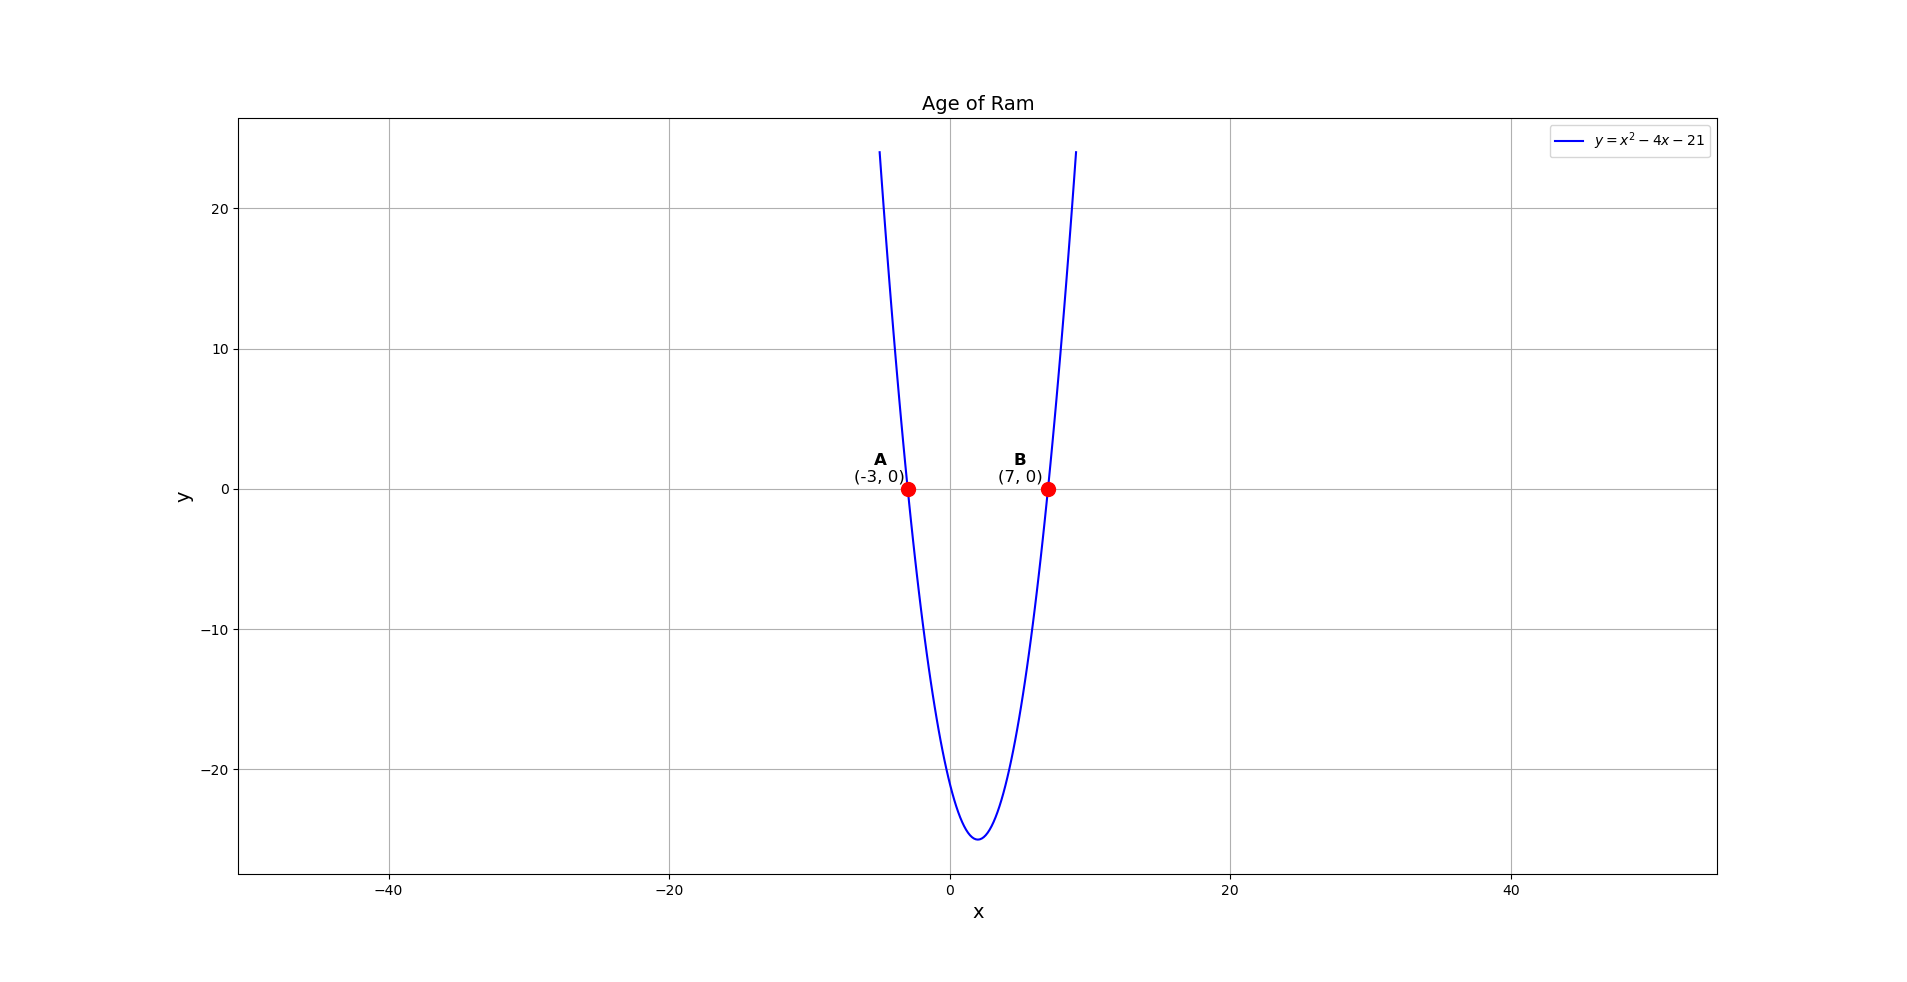
\includegraphics[width=0.7\columnwidth]{figs/fig1.png}
	\caption{}
   \label{}
\end{figure}
\end{frame}

\section{C Code}
\begin{frame}[fragile]
\frametitle{C Code}
\begin{lstlisting}[language=C]
#include <math.h>
void get_parabola_data(double* out_data) {
      double a = 1.0,b = -4.0,c = -21.0;
        double discriminant = sqrt(b*b - 4*a*c);
    double root1 = (-b + discriminant) / (2 * a);
    double root2 = (-b - discriminant) / (2 * a);
    out_data[0] = root1;
    out_data[1] = root2;
    int num_points = 101;
    out_data[2] = (double)num_points;
    int index = 3;
    for (int i = 0; i < num_points; i++) {
        double x = -5.0 + (14.0 * i) / (num_points - 1);
        double y = a*x*x + b*x + c;
        out_data[index] = x;
        out_data[index + 1] = y;
        index += 2;
    }
}

    \end{lstlisting}
\end{frame}

\section{Python Code}
\begin{frame}[fragile]
\frametitle{Python Code for Solving}
\begin{lstlisting}[language=Python]
import ctypes
import numpy as np

def get_data_from_c():

    lib = ctypes.CDLL('./code.so')

    data_size = 3 + 101 * 2
    double_array = ctypes.c_double * data_size
    lib.get_parabola_data.argtypes = [ctypes.POINTER(ctypes.c_double)]

    out_data_c = double_array()
    lib.get_parabola_data(out_data_c)

    return np.array(out_data_c)


\end{lstlisting}
\end{frame}

\begin{frame}[fragile]
\frametitle{Python Code for Plotting}
\begin{lstlisting}[language=Python]
# Code by /sdcard/github/matgeo/codes/CoordGeoVV Sharma
# September 12, 2023
# Revised July 21, 2024
# Released under GNU GPL
# Section Formula
import sys
sys.path.insert(0, '/workspaces/urban-potato/matgeo/codes/CoordGeo/')
import numpy as np
import matplotlib.pyplot as plt

from call import get_data_from_c
all_data = get_data_from_c()
num_points = int(all_data[2])
roots = all_data[0:2]
parabola_points = all_data[3:].reshape((num_points, 2))

positive_root = max(roots)
fig, ax = plt.subplots(figsize=(8, 8))
\end{lstlisting}
\end{frame}
\begin{frame}[fragile]
\frametitle{Python Code for Plotting}
\begin{lstlisting}[language=Python]
ax.plot(parabola_points[:, 0], parabola_points[:, 1], 'b-', label='$y = x^2 - 4x - 21$')
ax.scatter(roots, [0, 0], color='red', s=100, zorder=5)
pointA = np.array([min(roots), 0])
pointB = np.array([max(roots), 0])

label_A = f"$\\mathbf{{A}}$\n({pointA[0]:.0f}, {pointA[1]:.0f})"
ax.annotate(label_A,
            xy=pointA,
            xytext=(-20, 5),
            textcoords='offset points',
            ha='center',
            fontsize=12)
label_B = f"$\\mathbf{{B}}$\n({pointB[0]:.0f}, {pointB[1]:.0f})"
ax.annotate(label_B,
            xy=pointB,
            xytext=(-20, 5),
            textcoords='offset points',
            ha='center',

\end{lstlisting}
\end{frame}
\begin{frame}[fragile]
\frametitle{Python Code for Plotting}
\begin{lstlisting}[language=Python]
 fontsize=12)
 x.set_title("Age of Ram",fontsize=12)
ax.set_xlabel("x",fontsize=12)
ax.set_ylabel('y'.fontsize=12)

ax.grid(True)
ax.axis('equal')
ax.legend(loc='best')
plt.show()
\end{lstlisting}
\end{frame}
\end{document}
